%   % !TEX root = ../../VIII,3_Rahmen-TeX_8-1.tex
%
%
%   Band VIII, 3 N.~??A43/Y.9
%   Signatur/Tex-Datei: LH_35_09_14_003r
%   RK-Nr. 41150 (gänzlich) & 41151 (teilweise)
%   Überschrift: Invenire conoeides solidum, aequalis ubique resistentiae
%   Datierung: [März/April 1683 bis erste Hälfte 1684]
%   WZ: LEd-WZ 803009 = RK-WZ 358 (ein Fragment)
%.  SZ: (keins)
%.  Bilddateien (PDF): LH_35_09_14_003r_d1; LH_35_09_14_003r_d2; LH_35_09_14_003r_d3 (insgesamt: drei)
%
%
\selectlanguage{ngerman}%
\frenchspacing%
%
\begin{ledgroupsized}[r]{120mm}%
\footnotesize%
\pstart%
\noindent\textbf{Überlieferung:}%
\pend%
\end{ledgroupsized}%
\begin{ledgroupsized}[r]{114mm}%
\footnotesize%
\pstart%
\parindent -6mm
\makebox[6mm][l]{\textit{L}}%
Aufzeichnung:
LH~XXXV~9, 14 Bl.~3.
Ein halbes Blatt 4\textsuperscript{o},
am unteren Rand unregelmäßig beschnitten;
Fragment eines Wasserzeichens:
Papier aus dem Harz.
Eine Seite auf Bl.~3~r\textsuperscript{o};
Bl.~3~v\textsuperscript{o} überliefert das Teilkonzept N.~14\textsubscript{6},~\textit{L\textsuperscript{3}}.
Das Diagramm \lbrack\textit{Fig.~1}\rbrack\ % auf S.~\pageref{LH_35_09_14_003r_Fig.1}?? 
ist sowohl Bestandteil von N.~14\textsubscript{9} wie auch von N.~14\textsubscript{6},~\textit{L\textsuperscript{3}}.
\pend
\end{ledgroupsized}
%
% \vspace*{5mm}%
% \begin{ledgroup}%
% \footnotesize%
% \pstart%
% \noindent%
% \textbf{Datierungsgründe:}
% \pend%
% \end{ledgroup}%
%
%
\selectlanguage{latin}%
\frenchspacing%
%
%
%
\vspace*{8mm}
%
\count\Bfootins=1000
\count\Afootins=1200
\count\Cfootins=1000
%
%\count\Bfootins=1000
%\count\Cfootins=1000
%
\pstart%
\noindent%
%
\lbrack3~r\textsuperscript{o}\rbrack\ %%%% Blatt 3r
%
\pend%
\vspace{-0.5em}
%
\pstart%
\centering%
Invenire Conoeides Solidum,%
\protect\protect\index{Sachverzeichnis}{solidum conoeides}
aequalis ubique resistentiae%
\protect\index{Sachverzeichnis}{solidum ubique aequiresistens}%
\protect\index{Sachverzeichnis}{resistentia ubique aequalis}
\pend%
\vspace{0.5em}%
%
\pstart%
\noindent%
Sit Trilineum orthogonium planum \textit{ABCEA}%
\protect\index{Sachverzeichnis}{trilineum orthogonium}%
\protect\index{Sachverzeichnis}{trilineum planum}
quod rotatum circa proprium axem \textit{AB}
generet solidum conoeides \textit{AECDFA}.%
\protect\index{Sachverzeichnis}{solidum conoeides}
Hoc quaeritur tale,
%
\edtext{ut momentum\protect\index{Sachverzeichnis}{momentum solidi conoeidis}
portionis \textit{AEFA}}{%
\lemma{ut}\Bfootnote{%
\textit{(1)}~vires frangentes\protect\index{Sachverzeichnis}{vis frangens}
\textit{(2)}~momentum
\textit{(a)}~ipsius \textit{A}
\textit{(b)}~portionis \textit{AEFA}%
~\textit{L}}}
%
sit ad resistentiam suae basis \textit{EHF},\protect\index{Sachverzeichnis}{resistentia basis}
ut momentum totius \textit{ACDA}\protect\index{Sachverzeichnis}{momentum totius}
ad resistentiam suae basis \textit{CGD}.
Sunt autem resistentiae basium,\protect\index{Sachverzeichnis}{resistentia basis}
ut cubi diametrorum \textit{EF}, \textit{CD}.\protect\index{Sachverzeichnis}{cubus diametri}
Debet
%
\edtext{ergo linea}{%
\lemma{ergo}\Bfootnote{%
\textit{(1)}~figura
\textit{(2)}~linea%
~\textit{L}}}
%
\textit{AEC} esse talis,
ut
%
\edtext{momenta solidorum \textit{AEFA}, \textit{ACDA},%
\protect\index{Sachverzeichnis}{momentum solidi conoeidis}
sint ut cubi \textit{EF}, \textit{CD}, diametrorum basium.%
\protect\index{Sachverzeichnis}{cubus diametri}
\textit{CD} sit \textit{y}, \textit{AB} sit \textit{x}.}{%
\lemma{momenta}\Bfootnote{%
\textit{(1)}~frustroru
\textit{(2)}~sint ut cubi diametrorum basium
\textit{(3)}~\textit{AEF}
\textit{(4)}~solidorum \textit{AEFA}, \lbrack...\rbrack\ diametrorum basium. % \textit{ACDA}, sint ut cubi \textit{EF}, \textit{CD},
\textit{(a)}~\textit{EF} sit \textit{y}
\textit{(b)}~\textit{CD} sit \textit{y}, \textit{AB} sit \textit{x}.%
~\textit{L}}}
%
Et sit proprietas\protect\index{Sachverzeichnis}{proprietas curvae}
%
\edtext{curvae\protect\index{Sachverzeichnis}{curva} \textit{y} aequ. $x^{e}.$}{%
\lemma{curvae}\Bfootnote{%
\textit{(1)}~\textit{x}
\textit{(2)}~\textit{y} aequ. $x^{b}.$
\textit{(3)}~\textit{y} aequ. $x^{e}.$%
~\textit{L}}}
%
Et
\edtext{Elementa conoidis\protect\index{Sachverzeichnis}{elementum conoeidis}}{%
\lemma{Elementa}\Bfootnote{%
\textit{(1)}~cononoidis
\textit{(2)}~conoidis%
~\textit{L}}}
%
cum sint proportionalia ipsis \textit{yy},
erunt ut $x^{2e}.$
\edlabel{LH_35_09_14_003r_summasummarum_rglj-1}%
Quorum momenta\protect\index{Sachverzeichnis}{momentum solidi conoeidis}
ex \textit{CD} sunt summae
%
\edtext{summarum per
\edtext{alibi demonstrata,%
\edlabel{LH_35_09_14_003r_summasummarum_rglj-2}}{%
\lemma{alibi demonstrata}\Cfootnote{%
Siehe N.~14\textsubscript{8}, S.~\refpassage{LH_35_09_14_001r_summasummarum_ouir-1}{LH_35_09_14_001r_summasummarum_ouir-2}.}}
sunt autem}{%
\lemma{summarum}\Bfootnote{%
\textit{(1)}~sunt au
\textit{(2)}~per alibi demonstrata, sunt autem%
~\textit{L}}}
%
summae $\displaystyle x^{\frac{2e+1}{\cdot}}\! :\, \overline{2e +1}.$
Et summae summarum erunt:\protect\index{Sachverzeichnis}{summa summae}
$\displaystyle x^{\frac{2e+2}{\cdot}}\! :\, \overline{2e +1} \cdot \overline{2e +2}.$
Quae ut sint proportionales cubis ab \textit{y},
debent coincidere $y^3,$
seu $x^{3e},$
et $x^{2e+2}.$
Ergo aequantur $3e$
%
\edtext{et $2e+2,$
sive erit \textit{e} aequ. 2,}{%
\lemma{et}\Bfootnote{%
\hspace{-0,5mm}$2e+2,$
\textit{(1)}~sive \textit{e} et 2
\textit{(2)}~sive erit \textit{e} aequ. 2,%
~\textit{L}}}
%
et fiet \textit{y} aequ. $x^2.$
Ergo Conoeides parabolicum concavum%
\protect\index{Sachverzeichnis}{conoeides parabolicum concavum}
%
\edtext{seu Tuba parabolica\protect\index{Sachverzeichnis}{tuba parabolica}}{%
\lemma{seu}\Bfootnote{%
\hspace{-0,5mm}Tuba parabolica
\textit{erg.~L}}}
%
ubique aequaliter resistit.%
\protect\index{Sachverzeichnis}{solidum ubique aequiresistens}
Quae cum sit quinta pars cylindri circumscripti,%
\protect\index{Sachverzeichnis}{cylinder circumscriptus}
hinc
%
\edtext{modum}{%
\lemma{modum}\Bfootnote{%
\textit{erg.~L}}}
%
habemus
quo trabs\protect\index{Sachverzeichnis}{trabs ubique aequiresistens}
ad quintam ponderis\protect\index{Sachverzeichnis}{pondus trabis}
partem reduci potest,
%
\edtext{salva firmitate.\protect\index{Sachverzeichnis}{firmitas trabis}}{%
\lemma{salva}\Bfootnote{%
\textit{(1)}~resistentia
\textit{(2)}~firmitate%
~\textit{L}}}
%
\edtext{Quod Theorema pulcherrimum\protect\index{Sachverzeichnis}{theorema pulcherrimum}
a Galileo\protect\index{Namensregister}{\textso{Galilei} (Galilaeus, Galileus), Galileo 1564\textendash1642}
non fuit observatum.}{%
\lemma{Quod \lbrack...\rbrack\ observatum}\Cfootnote{%
Galilei hatte sich mit dem Längsschnitt eines prismatischen Balkens befasst, der an jedem Punkt seiner Länge den gleichen Bruchwiderstand aufweist.
Siehe G.~\textsc{Galilei}, \textit{Discorsi},
Leiden 1638, S.~137–141\cite{00050} (\textit{GO} VIII, S.~177–181).\cite{00048}}}
\pend%
%
%
  \newpage% 
%	% Diagramm Fig.~1
  \centerline{\includegraphics[width=0.36\textwidth]{gesamttex/edit_VIII,3/images/LH_35_09_14_003r_d1.pdf}}%
  \vspace*{0.5em}%
  \centerline{\lbrack\textit{Fig.~1}\rbrack}%
  \label{LH_35_09_14_003r_Fig.1}%
  \vspace{2.5em}%
%  \newpage%
%
%
% \vspace{2.0em}
\pstart%
\noindent%
% % % %    ACHTUNG GETRIXT: Folgende Cfootnote gehört zum Diagramm Fig.~1
\edtext{}{\lemma{\hspace{1,6mm}\lbrack\textit{Fig.~1}\rbrack}\killnumber\Cfootnote{%
Hierzu ist in \textit{L} ein gestrichener, hier nicht wiedergegebener Entwurf überliefert.
Das Diagramm gehört zugleich zum Teilkonzept N.~14\textsubscript{6},~\textit{L\textsuperscript{3}};
% (\textit{Demonstrationes novae de resistentia solidorum});
vgl. \lbrack\textit{Fig.~8a}\rbrack\ auf S.~\pageref{LH_35_09_14_003r_bis_Fig.8a}.}}%
%
\lbrack\textit{Unterhalb eines Trennungsstrichs:}\rbrack\
\pend%
\vspace{0.5em}
\pstart%
\noindent%
Solidum quaerere,
quod extremis apprehensum,
flectenti ubique aequaliter resistit.%
\protect\index{Sachverzeichnis}{solidum flectenti ubique aequiresistens}
\pend%
\count\Bfootins=1200
\count\Afootins=1200
\count\Cfootins=1200
%
%
\vspace{2.5em} 
\pstart 
\begin{minipage}[t]{0.5\textwidth}
\hspace{6mm}\includegraphics[width=0.67\textwidth]{gesamttex/edit_VIII,3/images/LH_35_09_14_003r_d2.pdf}
\end{minipage}
\hspace{7mm}
\begin{minipage}[t]{0.5\textwidth}
\includegraphics[width=0.66\textwidth]{gesamttex/edit_VIII,3/images/LH_35_09_14_003r_d3.pdf}
\end{minipage}
\\
\\
\hspace*{27mm} [\textit{Fig.~2a}] \label{LH_35_09_14_003r_Fig.2}\hspace*{56mm} [\textit{Fig.~2b}]\label{LH_35_09_14_003r_Fig.3}
\pend
%\vspace{1em}
%
%
%%  \newpage% 
%  \vspace{2.5em}%	% Diagramm Fig.~2a
%  \centerline{\hspace*{-60mm}\includegraphics[width=0.3\textwidth]{gesamttex/edit_VIII,3/images/LH_35_09_14_003r_d2.pdf}}%
%  \vspace*{0.5em}
%  \centerline{\hspace*{-60mm}\lbrack\textit{Fig.~2a}\rbrack}%
%  \label{LH_35_09_14_003r_Fig.2}%
%%  \vspace{1.5em}%
%%  \newpage%
%%
%%  \newpage% 
%  \vspace{-7.25em}%	% Diagramm Fig.~3
%  \centerline{\hspace*{60mm}\includegraphics[width=0.3\textwidth]{gesamttex/edit_VIII,3/images/LH_35_09_14_003r_d3.pdf}}%
%  \vspace*{0.5em}
%  \centerline{\hspace*{60mm}\lbrack\textit{Fig.~2b}\rbrack}%
%  \label{LH_35_09_14_003r_Fig.3}%
%%  \vspace{1.5em}%
%%  \newpage%
%%
%
%    %    %    %    Ende des Textes auf Blatt 3r
%
%